\chapter{Numerical Simulation of Electroosmosis using OpenFOAM}
\label{chpt:numerical}
\section{Introduction}
In Chapter \ref{chpt:zero_thickness}, \ref{chpt:finite_thickness} and \ref{chpt:eddies}, we introduced numerical simulations of electroosmotic flow in a nanopore system under different conditions. The numerical simulations were carried out using a solver created in OpenFOAM. 

OpenFOAM is an open source CFD library \cite{OPENFOAM} designed for computational mechanics. It is based on the finite volume method, which we use to discretize the PNP-Stokes equations. OpenFOAM contains a collection of well-designed object-oriented classes to represent mesh, fields, vectors, tensors and matrices, as well as operators on fields and tensors, like the Laplace operator and the divergence operator. The discretized matrix equation is solved using the provided OpenFOAM linear solver. For the current applications, a bi-conjugate gradient stabilized (BiCGSTAB) solver is used. OpenFOAM also contains tools for pre-processing and post-processing.

\section{PNPStokesFoam - An OpenFOAM solver for PNP-Stokes system of equations in nanopores}
The steady state PNP-Stokes system of equations given in previous chapters are re-written below for completeness of this chapter. 
\begin{eqnarray}
\epsilon \nabla^2 \phi + \sum_{i=1}^{N} z_ien^i & = & 0,
\label{eq:poisson_num}
\\
\nabla\cdot\left\lbrack n^i\mathbf{u} -\omega^i(kT\nabla
n^i + ez_in^i\nabla\phi) \right\rbrack&=&0 ,
\label{eq:NP_num}
\\ 
-\nabla p + \mu \nabla^2 \mathbf{u} -  \nabla \phi \sum_{i=1}^{N} z_ien^i & = & 0, \label{eq:stokes_num}\\
\nabla \cdot \mathbf{u} & = & 0. \label{eq:continuity_num}
\end{eqnarray} 

The set of equations are coupled and need to be solved in an iterative manner. 

By convention, OpenFOAM solvers are named by ``-Foam''. We hence call our solver PNPStokesFoam. The details of the solvers are explained as follows.

\subsection{The Poisson-Nernst-Planck equations}
\subsubsection{Convection-diffusion equations of ionic species}
Equation \ref{eq:NP_num} is the Nernst-Planck equation for ionic species $n^i$. It is a convection-diffusion equation. Let us first assume that the flow field $\mathbf{u}$ and electric potential $\phi$ is known. The convective fluxes include the electrophoretic  $(-\omega^iz_ie\nabla\phi)n^i$ and advective $\mathbf{u}n^i$ contributions. The finite volume method is used to discretize Equation \ref{eq:NP_num}. Part of the pseudo code is reproduced here in order to illustrate:

\begin{lstlisting}
surfaceScalarField rhoFluxi    // define electrophoretic velocity
(
	-zi*(Di/kB/T)*e*fvc::snGrad(phiV)*mesh.magSf()
);

ni.boundaryField().updateCoeffs();    // apply boundary condition

fvScalarMatrix niEqn    // assemble matrix equation
(
    fvm::div(rhoFluxi, ni) + fvm::div(phi,ni) - fvm::laplacian(Di, ni)
);  
      
niEqn.relax();    // apply under-relaxation
niEqn.solve();    // solve using provided linear solver
\end{lstlisting}

\textsf{surfaceScalarField} is the name of the C$++$ class provided by OpenFOAM for a scalar field defined at the control volume faces. An object \textsf{rhoFluxi} of class \textsf{surfaceScalarField} is defined and calculated as the multiplication of electrophoretic velocity $(-\omega^iz_ie\nabla\phi)$ and the control volume face area \textsf{mesh.magSf()}. Here \textsf{fvc::snGrad(phiV)} stands for the finite volume operator of surface normal gradient \textsf{fvc::snGrad} acting on the scalar field \textsf{phiV} ($\phi$). \textsf{fvc::snGrad(phiV)} is calculated explicitly using known values of $\phi$. 

Similarly multiplication of convective velocity $\mathbf{u}$ and control volume face area \textsf{mesh.magSf()} gives another object of class \textsf{surfaceScalarField}. We call it \textsf{phi}.

Now we are ready to discretize Equation \ref{eq:NP_num}. \textsf{fvScalarMatrix} is a class provided by OpenFOAM for a linear equation of a scalar (matrix equation). An object \textsf{niEqn} of class \textsf{fvScalarMatrix} is defined. This is the linear equation we get from discretization. In line 10, the operator \textsf{fvm::div} is the implicit finite volume operator for $\nabla \cdot$, while the operator \textsf{fvm::laplacian} is the finite volume operator for $\nabla^2$. Line 10 therefore corresponds to Equation \ref{eq:NP_num} in the OpenFOAM syntax. 

The discretization operators \textsf{fvm::laplacian} and \textsf{fvm::div} discretize Equation \ref{eq:NP_num} using the discretization scheme specified by user in an input file. For the applications of interest, the Peclet number is usually large, therefore we use second-order upwind scheme for convective terms. We also use central difference scheme for diffusive terms.

After the matrix equation has been assembled, under-relaxation is applied, as we are solving a nonlinear system. \textsf{niEqn.solve()} solves this linear equation using the linear solver provided. For the current applications, a bi-conjugate gradient stabilized (BiCGSTAB) solver is used. The relaxation factor and choice of linear solver can be specified in an input file.

\subsubsection{Electric potential}
We solved the Nernst-Planck equation assuming that the potential $\phi$ is known. However, $\phi$ needs to be solved from Equation \ref{eq:poisson_num}, which contains $n^i$ at the right hand side. Equation \ref{eq:NP_num} and \ref{eq:poisson_num} are therefore coupled and need to be solved iteratively.

In this step, we assume that the ionic concentrations $n^i$ is known. In the current application we have 2 ionic species.

The pseudo code for solving Equation \ref{eq:poisson_num} is illustrated below.

\begin{lstlisting}
solve
(
    -fvm::laplacian(phiV) == e*(z1*n1+z2*n2)/(ep0*epr)    // RHS is the local charge density
);
phiV.relax();    // apply under-relaxation
\end{lstlisting}

The local charge density is calculated explicitly as \textsf{e*(z1*n1+z2*n2)}. This code corresponds to Equation \ref{eq:poisson_num} in an OpenFOAM syntax. The \textsf{fvm::laplacian} discretizes the unknown \textsf{phiV} according to user-specified scheme (central difference). The resulting linear equation is solved by \textsf{solve()} operator, again using a user-specified linear solver.

\subsection{Stokes equation}
\subsubsection{Momentum equations}
Once we have a relatively good prediction for $n^i$ and $\phi$, we can update the flow field to take into account the electric body force $-e\sum_i(z_in^i)\nabla\phi$. The pseudo code for the momentum equation is illustrated below.

\begin{lstlisting}
fvVectorMatrix UEqn
(
    -fvm::laplacian(mu, U)    // assemble matrix for the momentum equation
);
UEqn.relax();

solve
(
    UEqn == 
	- fvc::grad(p)    // pressure gradient 
	- e*(z1*c1+z2*c2)*fvc::grad(phiV)    //
);
\end{lstlisting}

\textsf{UEqn} is an object of OpenFOAM class \textsf{fvVectorMatrix}, which is the matrix equation for a vector. This class is similar to \textsf{fvScalarMatrix} only that it is for a vector equation (as opposed to that for a scalar). Again, operator \textsf{fvm::laplacian} accepts different discretization schemes specified by user at runtime in the input file. The source term for momentum equation includes the pressure gradient, and the electric body force, which is calculated explicitly using the most updated $n^i$ and $\phi$ as \textsf{- e*(z1*c1+z2*c2)*fvc::grad(phiV)}. Here the OpenFOAM operator \textsf{fvc::grad} calculates the gradient of its argument at control volume centers explicitly. This corresponds to Equation \ref{eq:stokes_num} in OpenFOAM syntax.

\subsubsection{SIMPLE algorithm}
Due to the incompressibility of the water, we need to take care of the pressure-velocity coupling. We adopt the SIMPLE algorithm on a collocate grid with the Rhie-Chow interpolation. The pseudo code is illustrated below.

\begin{lstlisting}
volScalarField rAU(1.0/UEqn.A());    // A^{-1}

U = rAU*(UEqn.H() - e*(z1*c1+z2*c2)*fvc::grad(phiV));    // U^*
    
phi = fvc::interpolate(U) & mesh.Sf();    

fvScalarMatrix pEqn
(
    fvm::laplacian(rAU, p) == fvc::div(phi)    // pressure Poisson equation
);
pEqn.setReference(pRefCell, pRefValue);    // set reference value for pressure

pEqn.solve();    // solve pressure equation

phi -= pEqn.flux();
p.relax();
U -= rAU*fvc::grad(p);    // correct velocity field
\end{lstlisting}

The pseudo code corresponds to the following algorithm:
\begin{equation}
A \mathbf{U} = \mathbf{H} - \nabla p + \mathbf{f}
\label{eq:SIMPLE1}
\end{equation}
Here $A$ is the diagonal component of matrix \textsf{UEqn}. $\mathbf{H}$ is the off-diagonal terms of the matrix equation. $\mathbf{f}$ stands for body force other than gradient of pressure. In our case it is the electric force. From the momentum equation we have solved for $\mathbf{U}$. However it in general does not satisfy continuity. We now use the continuity equation to correct flow field to make it divergence free.

From Equation \ref{eq:SIMPLE1} we have 
\begin{equation}
\mathbf{U} = A^{-1}(\mathbf{H}+\mathbf{f}) - A^{-1}\nabla p
\label{eq:SIMPLE2}
\end{equation}
Let us call $A^{-1}(\mathbf{H}+\mathbf{f})$ as $\mathbf{U}^*$. If we apply the divergence operator to both sides of Equation \ref{eq:SIMPLE2}, and force $\mathbf{U}$ to satisfy continuity, then we get
\begin{equation}
\nabla \cdot \left(A^{-1}\nabla p\right) = \nabla \cdot \mathbf{U}^*
\label{eq:SIMPLE3}
\end{equation}

From Equation \ref{eq:SIMPLE3} we calculate $p$ and correct the velocity $\mathbf{U}$ to be $\mathbf{U}^* - A^{-1}\nabla p$. This will ensure that the corrected velocity field satisfies the incompressibility constraint.

The algorithm outlined above is essentially the SIMPLE (Semi-Implicit Method for Pressure Linked Equations) algorithm with Rhie-Chow interpolation on a collocated grid. $A^{-1}$ is \textsf{rAU} in the code. Matrix equation \textsf{pEqn} corresponds to Equation \ref{eq:SIMPLE3}.

\subsection{Segregated Solver}
We set up a segregated solver to solve the PNP-Stokes equations. We start from a zero flow field. Equations  (\ref{eq:poisson_num}) and (\ref{eq:NP_num}) are solved sequentially and we iterate with under-relaxation until the residual is small. Under--relaxation is necessary because the PNP system is coupled. 

The electric volume force $- \nabla \phi\sum_i z_ien^i $ is obtained from this solution and used explicitly in the next step viz. the solution of the incompressible Stokes flow: Equations (\ref{eq:stokes_num}) and (\ref{eq:continuity_num}). The electric force term is regarded as given when solving for the flow. The SIMPLE algorithm is again iterative, and we iterate until the residual is small.

The flow field is then substituted into (\ref{eq:NP_num}) and the PNP system is solved once again using the updated flow field. After $n^i$ and $\phi$ are updated, we compute the new electric force term, and solve for the new flow field.

An outer loop is constructed to iterate over the PNP and Stokes flow modules that run sequentially.

\subsection{Boundary conditions}
OpenFOAM provides a collection of built-in boundary conditions such as the Dirichlet boundary condition and the Neumann boundary condition. These boundary conditions can be used in different contexts for different physical conditions.

A schematic view of the axisymmetric geometry used for the full numerical simulations is provided in Figure \ref{fig:system_num}. 
\begin{figure}[h]
\centering
\includegraphics[width=1.0\textwidth]{openfoam/figure4.eps}
\caption{A typical nanopore geometry of interest}
\label{fig:system_num}
\end{figure}
It consists of a circular hole of radius $a$ in a solid dielectric membrane CDEF of arbitrary thickness $h\ge 0$. This geometry can be created using an OpenFOAM script called \textsf{blockMesh}. The coordinates of the vertices, the edges and the number of elements along each edge are needed. \textsf{blockMesh} then generates a structured mesh to be used by OpenFOAM solver.

The membrane surfaces CD, DE and EF have a uniform surface charge density $\sigma$. Two large cylindrical reservoirs are connected to the pore, one at each end. In our simulation we consider a 1-1 symmetric electrolyte solution containing ions with equal mobilities. Note the length and radius of both the reservoirs are identical, and are $L_R=\max(10a, 10\kappa^{-1})$, chosen to be much larger than either the hole radius $a$ or the Debye length $\kappa^{-1}$  in order to approximate an infinite reservoir. 

We adopt the following boundary conditions \cite{Mao2013}. The ion number densities on AB and GH are constant, and equal to the number density $n_\infty$ in the bulk solution far from any charged surfaces. The electrical potentials are uniform on AB and on GH, with a potential difference of $\Delta\phi$ between the top (AB) and bottom (GH). The pressure $p_{\infty}$ on AB is uniform and equal to that on GH. On the side walls BC and FG, the radial electric field, ionic flux and radial velocity, which decay away from the pore, are set to zero. A zero tangential shear stress is imposed on flow parallel to the side walls. At the membrane surfaces CD, DE and EF, a no--flux condition is used for Equation (\ref{eq:NP}) and a no--slip condition for the flow. 

All the boundary conditions mentioned above can be easily implemented using the OpenFOAM built-in boundary conditions or 3-rd party boundary condition \textsf{groovyBC}. \textsf{groovyBC} is a 3-rd party extension of the standard OpenFOAM boundary conditions that can handle Robin-type conditions.

The electrostatic boundary condition at membrane surfaces CD, DE and EF needs special treatment.

\subsubsection{Electrostatic boundary condition}
The electric field $\mathbf{E}$ undergoes a jump across the solid membrane-fluid interface such that
$\epsilon \mathbf{E} \cdot  \hat{\mathbf{n}} - \epsilon_{s} \mathbf{E}_{s} \cdot \hat{\mathbf{n}} = \sigma$ 
where $\epsilon$ is the electrical permittivity of the fluid and $\epsilon_{s}$ is the permittivity of the membrane, $\mathbf{E}_{s}$ is the electric field at the interface within the membrane and $\hat{\mathbf{n}}$ is the unit normal at the surface directed into the fluid. The potential $\phi$ is continuous across the interface. 

If the membrane polarizability is sufficiently small that $|\epsilon_{s} \mathbf{E}_{s} \cdot \hat{\mathbf{n}}|\ll|\epsilon \mathbf{E} \cdot  \hat{\mathbf{n}}|$, then the jump condition of the normal component of the field may be replaced by $\epsilon \mathbf{E} \cdot \hat{\mathbf{n}} = \sigma$. This approximation is often justified because the dielectric constant of water ($80$) greatly exceeds that of common substrate materials (plastics, silica, lipids etc.) which are typically of order unity. Formally, this is equivalent to assuming ``$\epsilon_s = 0$ which of course should not be interpreted literally as no physical material can have a relative permittivity less than unity! In this case, the electrostatic boundary condition reduces to specifying the normal gradient of $\phi$ at the boundary. This inhomogeneous Neumann boundary condition can be conveniently implemented using the OpenFOAM built-in boundary conditions or \textsf{groovyBC}. We have shown in Chapter \ref{chpt:zero_thickness} that assuming $\epsilon_s=0$ has little effect on the total electroosmotic flow through the nanopore when $\sigma \neq 0$. The biggest advantage of applying this assumption is that the computational domain may be restricted to include only the fluid phase.

On the other hand, when $|\epsilon_{s} \mathbf{E}_{s} \cdot \hat{\mathbf{n}}|$ and 
$|\epsilon \mathbf{E} \cdot  \hat{\mathbf{n}}|$ become comparable, such as when $\sigma = 0$ and ICEO is the primary mechanism of interest, we need the full jump conditions of $\mathbf{E}$ as the electrostatic boundary condition. In this case, the flow is driven by the ICEO effect. We have studied eddies within uncharged nanopores due to ICEO in Chapter \ref{chpt:eddies}. 

It should be noted here that when the full jump condition of $\mathbf{E}$ is used, \textsf{nppStokesFoam} needs to be modified to include the solid region, where the net charge density is zero. Hence, instead of solving Equation \ref{eq:poisson_num} for $\phi$ in the fluid region alone, we need to solve Equation \ref{eq:poisson_num} together with a Laplace equation
\begin{equation}
\epsilon_s \nabla^2 \phi = 0 \qquad \mbox{within membrane}
\label{eq:laplace_num}
\end{equation}
and the coupling condition of $\epsilon \mathbf{E} \cdot  \hat{\mathbf{n}} - \epsilon_{s} \mathbf{E}_{s} \cdot \hat{\mathbf{n}} = \sigma$ at the solid-fluid interface. 

A separate solver \textsf{mrnppStokesFoam} is developed in OpenFOAM to account for this change; here \textsf{mr} stands for multi-region. The coupling boundary condition is not provided in standard OpenFOAM in the context of electrostatics. However, OpenFOAM does provide a built-in template for thermal boundary conditions at the solid-fluid interface in the context of conjugate heat transfer problems. Exploiting the fact that electrostatics and heat conduction are described by identical equations, a new OpenFOAM boundary condition is developed using the OpenFOAM template for heat conduction.

The OpenFOAM template relates the value at boundary $T_f$ and the value at the neighboring control volume center $T_c$ (see Figure \ref{fig:CV}) as follows:
\begin{equation}
T_f = f\cdot \mathsf{refValue} + (1-f)\cdot(T_c + \mathsf{refGrad}\cdot\delta)
\label{eq:OF_BC}
\end{equation}
Here $\delta$ is the distance between control volume center and face center, $f$ is a user defined interpolation factor. \textsf{refValue} and \textsf{refGrad} are defined by the user to implement different forms of flux-type boundary conditions.

\begin{figure}[h]
\centering
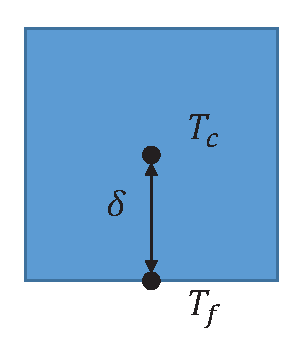
\includegraphics[scale=0.5]{openfoam/CV1.eps}
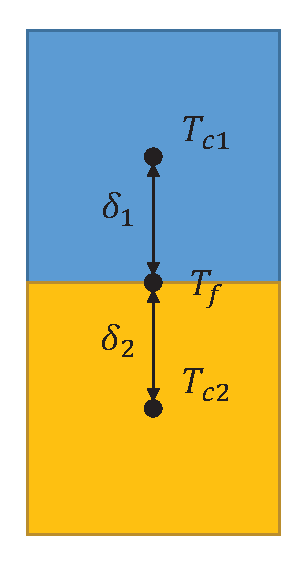
\includegraphics[scale=0.5]{openfoam/CV.eps}
\caption{Control volume (left) adjacent to a boundary and (right) at solid(yellow)-fluid(blue) interface}
\label{fig:CV}
\end{figure}


For a solid-fluid interface shown in Figure \ref{fig:CV}, according to Gauss theorem, we have a discretized form as follows:
\begin{equation}
\epsilon_1 \frac{T_f-T_{c1}}{\delta_1} + \epsilon_2 \frac{T_{c2}-T_f}{\delta_2} = \sigma
\label{eq:OF_BC1}
\end{equation}
Here $\epsilon_1$ and $\epsilon_2$ are permittivities of regions 1 and 2, respectively, and $\sigma$ is the surface charge density. Re-arranging Equation \ref{eq:OF_BC1} we get
\begin{equation}
T_f = \left(\frac{\epsilon_1}{\delta_1}+\frac{\epsilon_2}{\delta_2}\right)^{-1} \left( \frac{\epsilon_1}{\delta_1}T_{c1}+\frac{\epsilon_2}{\delta_2}T_{c2}+\sigma\right)
\label{eq:OF_BC2}
\end{equation}

In order to relate $T_{c1}$ and $T_f$, we define $f = \left(\frac{\epsilon_1}{\delta_1}+\frac{\epsilon_2}{\delta_2}\right)^{-1}\frac{\epsilon_2}{\delta_2}$, \textsf{refValue}$=T_{c2}$ and \textsf{refGrad}$=\frac{\sigma}{\epsilon_1}$ in Equation \ref{eq:OF_BC} which reproduces Equation \ref{eq:OF_BC2}. 

The pseudo code is illustrated below.

\begin{lstlisting}
this->refValue = nbrT;

this->refGrad = surfCharge / myEps;

this->f = nbrKDelta / (nbrKDelta + myKDelta);
\end{lstlisting}
For control volume 1, control volume 2 is its neighbor across the interface, hence $T_{c2}$ is \textsf{nbrT} in the code. 
Furthermore, $\epsilon_1$ is \textsf{myEps}, $\sigma/\delta$ is called \textsf{KDelta} in the code, and $\sigma$ \textsf{surfCharge}.

For control volume 2, the same self-neighbor relation holds. The code does not need to be modified.

\section{Concluding remarks}
We have used the OpenFOAM CFD library to develop solvers for PNP-Stokes equations. The finite volume method is used to discretize the governing equations. The discretized equations are then solved iteratively due to multiphysics coupling and velocity-pressure coupling. These solvers have been applied successfully to simulations of nanopore problems described in previous chapters. Both qualitative and quantitative agreements have been reached.

OpenFOAM provides templates for solvers and boundary conditions. These templates are modified by the author to create new solvers and boundary conditions suitable for the problems of interest. For instance, the jump condition of the electric field at solid-fluid interface is created in analogy to OpenFOAM thermal boundary conditions in conjugate heat transfer problems. In addition, OpenFOAM has large collections of third-party extension due to its popularity in the CFD community. We have used the \textsf{groovyBC} (part of the \textsf{swak4Foam} extension) created by Dr. Bernhard Gschaider. Here we thank the OpenFOAM community for sharing these powerful tools. 

The author also thanks Dr. Neelesh Patankar for helpful guidance and discussions on finite volume method and CFD.
